\chapter{手法}
本論文の問題はニューロンのクラスタリングである.
ニューロン間の類似度$A \in [0, 1]^{I \times I}$をクラスタリングする問題を解く.
ただし,$I$はニューロン数で$a_{ij}$はニューロン$i$と$j$の類似度である.
本章では$A$の推定方法とクラスタリング手法の説明をする.

$A$は非負行列因子分解(NMF)で推定する.
NMFを使う理由は数理モデルに基づいており,次節で説明する.
クラスタリング手法にはスペクトラルクラスタリングを用いる.
スペクトラルクラスタリングはグラフカットとして解釈でき,類似度行列$A$をクラスタリングするのに適している.

\section{類似度$A$の推定}
本節ではNMFとブートストラップ法によって類似度$A$を推定する方法を述べる.
観測データ$X$は$X \in \mathbb{R}_+^{I \times J}$とする.
ただし,$\mathbb{R}_+$を非負の実数の集合,$J$を観測時系列の長さとする.
% ある行列$A$の$i$行を$a_{i:}$,$j$列を$a_{:j}$,$(i,j)$要素を$a_{ij}$または$[A]_{ij}$と表記する.
NMFで推定するのは$A^* \in \{0,1\}^{I \times I}$であり,$a^*_{ij}$はニューロン$i$とニューロン$j$が同じグループに所属するか否かを表す.
ブートストラップ法を用いて類似度$A = E[A^* | X]$を推定する.
$A$の要素$a_{ij}$はニューロン$i$とニューロン$j$が同じグループである確率$Pr(a_{ij} = 1)$を意味する.

\subsection{数理モデル}
カルシウムイメージングデータに対していくつかの仮定をおいた.
\\ \\
\noindent \textbf{仮定 1}\\
グループが$K$個存在し,同じグループ内のニューロンは同時に活動する.
ニューロンは複数のグループに所属することができる.
観測時間内ではグループに属するニューロンは変化しない.
\\ \\
\textbf{仮定 2}\\
複数のグループが同時に活動する時,属するニューロンは被らない(ニューロンが属するグループは同時には活動しない).
\\

これらの仮説をもとに,数理モデルを構築する.
ニューロン$i$の観測時系列は$x_{i:} \in \mathbb{R}_+^{J}$である.

$c_{k:} \in \mathbb{R}^J_+$ ($k=1,\dots,K$)をグループ$k$の活動の時系列とすると,仮定より$x_{i:}$は$c_{i:}$の重み付き和として表す:
\begin{equation}
	x_{i:} = \sum_{k=1}^K d_{ik} c_{k:} + \eta_{i:},
  \label{eq:x}
\end{equation}
ただし,$d_{ik} \in \mathbb{R}^+$で,$\eta_{i:} \in \mathbb{R}^J$はガウスノイズの時系列である.
カルシウムイメージングのノイズはポアソン分布に従う光子ノイズであるが,光子数が多い場合はガウス分布で近似できる~\cite{Sjulson2007}.

仮定2を置くことによって,\eqref{eq:x}の線形モデルを考えることができる.
仮定2がなかった場合,あるニューロンの蛍光強度は複数グループからの影響によって上限なく上昇できてしまう.
実際は,ニューロンの蛍光強度の最大値は蛍光タンパク質の量で決まるため,蛍光強度は最大値で飽和する.
その場合\eqref{eq:x}には飽和を組み込まなければいけない.
本論文では,複数グループが同時に活動する場合はそれらも同じグループとみなし,単純な線形モデルで表す.

\eqref{eq:x}は行列形式で以下のように表現できる:
\begin{align}
  Y &= DC, \\
  X &= Y + H. \label{eq:model_matrix}
\end{align}
ただし,$D \in \mathbb{R}_+^{I \times K}$, $C \in \mathbb{R}_+^{K \times J}$, $H \in \mathbb{R}^{I \times J}$である.
また,$D$の要素$(i,k)$は$d_{ik}$,$C$の$i$行は$c_{i:}$,$H$の$i$行は$\eta_{i:}$である.

\subsection{NMFによる$A^*$の推定}
非負行列因子分解(nonnegative matrix factorization; NMF)\cite{Lee1999}は行列分解の手法の一つである.
NMFは以下の最適問題を解く:
\begin{equation}
	\argmin_{D \geq 0, C \geq 0} ||X - Y||_F^2.
\end{equation}

基底数$k$のNMFのモデルを$\mathcal{M}_k$とおく.
ノイズ行列$H$の各要素が正規分布$\mathcal{N} (0, \sigma^2)$に従う$\mathcal{M}_k$の尤度は以下である.
\begin{align}
	p(X | Y_k, \mathcal{M}_k) = \prod_{i,j} \frac{1}{\sqrt{2 \pi \sigma^2}} \exp(-\frac{([Y_k]_{ij} - x_{ij})^2}{2 \sigma^2}),
\end{align}
ただし,$Y_k$はモデル$\mathcal{M}_k$における推定量である.
対数尤度は以下のようになる.
\begin{align}
	\log p(X | Y_k, \mathcal{M}_k) = - \frac{IJ}{2} (\log 2\pi + 2 \log \sigma) - \frac{1}{2 \sigma^2} \sum_{ij}([Y_k]_{ij} - x_{ij})^2.
\end{align}

NMFの寄与率行列$P \in \mathbb{R}^{I \times K}$の要素を次のように定義する:
\begin{align}
	p_{ik} &= \frac{||d_{ik} c_{k:}||_1}{\sum_{l=1}^K || d_{il} c_{l:} ||_1} \\
	&= \frac{d_{ik} || c_{k:} ||_1}{ \sum_{l=1}^K d_{il} || c_{l:} ||_1 }.
\end{align}
要素$p_{ik}$はニューロン$i$に対する基底$k$の寄与率という意味である.

$A^*$は寄与率行列$P$から作成する.
まず,$P$と同じサイズの行列$G \in \{0, 1\}^{I \times K}$を作る.
$G$は,$P$の各行について最大値のみを$1$,それ以外を$0$とした行列である.
\begin{align}
	g_{ij} = \begin{cases}
		1 & (j = index(max(p_{i:}))) \\
		0 & (otherwise)
	\end{cases}
\end{align}
% まず,以下の手順で$P$と同じサイズの行列$G \in \{0, 1\}^{I \times K}$を作る.
% $p_{i:}$の累積寄与率を$F_i$とおく.
% $F_i$は$p_{i:}$を大きい順に足した関数である.
% 閾値を$threshold$とおき,$F_i < threshold$となる$p_{i:}$のインデックスを$index$とおく.
% $p_{i:}$に該当する$g_{i:}$を
% \begin{align}
% 	g_{ij} = \begin{cases}
% 		1 & (j \in index) \\
% 		0 & (otherwise)
% 	\end{cases}
% \end{align}
% と定義する.

推定量$A^*$を
\begin{align}
	A^* = G G^{\top},
\end{align}
と定義する.

この推定量はcluster ensembleでも用いられているpairwise similarity\cite{Boongoen2018}と似たものになっている.

\subsection{NMFの一意性}
NMFの推定には一意性がなく,ある正則行列$Q$を考えた時,
\begin{align}
	X &= DC \\
	&= D Q R C \label{eq:dqrc} \\
	&= D'C', \\
	R &= Q^{-1}, \\
	D' &= DQ, \\
	C' &= RC,
\end{align}
のように別の$D'$と$C'$が推定される可能性がある.

NMFに一意性がある条件は\cite{Fu}などでまとめられている.
しかし,一意性を持たせるにはかなり条件が狭められる.

NMFと同じように非負行列を分解する手法にnonnegative rank factorization (NRF)~\cite{Dong2014}がある.
NRFではデータ行列$X$を$X = DC$に分解できる最小の基底数をnonnegative rank $\text{rank}_+(X)$と定義し,$\text{rank}(X) = \text{rank}(X)_+$となる行列$X$を対象とする.
全ての非負行列はNMFできるが,NRFができるとは限らない.
NRFの計算はNP困難であるが,\cite{Dong2014}ではNRFの計算と,NRFを持たない行列に対してMNRSという分解の計算方法を提示している.
しかし,$X$にノイズが乗っている場合にNRFが存在する条件は調査されていない.

この場合の$D'$と$C'$を用いて作られる寄与率行列$P'$と元の寄与率行列$P$の関係を考える.
% 要素$p'_{ik}$の分子は,$D'$と$C'$が正であることを用いて
% \begin{align}
% 	d'_{ik} ||c'_{k:}||_1 &= \left( \sum_{l = 1}^K d_{il} q_{lk} \right) \left( \sum_{m = 1}^K r_{km} ||c_{m:}||_1 \right) \\
% 	&= \sum_{m = 1}^K \left( d_{i1} q_{1k} r_{km} + \cdots + d_{iK} q_{Kk} r_{km} \right) ||c_{m:}||_1,
% \end{align}
% である.
% 分母を考えると,
% \begin{align}
% 	\sum_{l=1}^K d'_{il}||c'_{l:} ||_1 &= \sum_{l = 1}^K \sum_{m = 1}^K \left( d_{i1} q_{1l} r_{lm} + \cdots + d_{iK} q_{Kl} r_{lm} \right) ||c_{m:}||_1 \\
% 	&= \sum_{m = 1}^K \left( d_{i1} \sum_{l = 1}^K q_{1l}r_{lm} + \cdots d_{iK} \sum_{l = 1}^K q_{Kl} r_{lm}\right) ||c_{m:}||_1
% \end{align}
% \eqref{eq:dqrc}より,
% \begin{align}
% 	\sum_{l = 1}^{K} q_{il} r_{lj} = \begin{cases}
%     1 & (i = j) \\
%     0 & (otherwise)
%   \end{cases}
% \end{align}
% なので,
% \begin{align}
% 	\sum_{l=1}^K d'_{il} || c'_{l:} ||_1 &=& \sum_{m = 1}^K d_{im} ||c_{m:}||_1,
% \end{align}
% となり,$p_{ik}$と$p'_{ik}$の分母は一致する.
% 寄与率$p'_{ik}$は,
% \begin{align}
% 	p'_{ik} &= \frac{ d'_{ik} || c'_{k:}||_1 }{ \sum_{m = 1}^K d'_{im} || c'_{m:}||_1 } \\
% 	&= \frac{\sum_{l = 1}^K d_{il} q_{lk}}{\sum_{m=1}^K d_{im} || c_{m:} ||_1} ||c'_{k:}||_1 \\
% 	&= ||c'_{k:}||_1 \sum_{l = 1}^K \frac{d_{il}}{\sum_{m=1}^K d_{im} || c_{m:} ||_1} q_{lk} \\
% 	p_{il} = \frac{d_{il} ||c_{l:}||_1 }{ \sum_{m = 1}^K d_{im} || c_{m:} ||_1 } \text{より,} \\
% 	&= ||c'_{k:}||_1 \sum_{l = 1}^K \frac{p_{il}}{ ||c_{l:}||_1 } q_{lk}\\
% 	&= \sum_{l = 1}^K \frac{ ||c'_{k:}||_1 }{ ||c_{l:}||_1 } q_{lk} p_{il}
% \end{align}
% となる.
% これより,
% \begin{align}
% 	P' &= PV, \\
% 	V &\in \mathbb{R}^{K \times K}, \\
% 	v_{ij} &= \frac{ || c'_{j:} ||_1 }{|| c_{i:} ||_1} q_{ij},
% \end{align}
% と表せることから,$P'$は$P$を変換した行列であることがわかる.
% この変換によって異なるニューロンの寄与率は同じだけ変化する.
簡単のため,$X$に行和$1$の正規化を加え$C$に行和$1$の制約を加える.
この時$D$の行和も$1$となり,$P = D$となる.
\eqref{eq:dqrc}より,$P' = PQ$となる.
この時,$G$の作り方には一意性がないため推定量$A$にも一意性がない.

$K=3$の場合の図を用いて説明をする.
\Figref{fig:d-space}に$C$の空間内の$x_{i:}$と$D$の空間内の$d_{i:}$を表す.
$d_{i:}$の和は$1$であるが,軸は\Figref{fig:p-rotate}のように動くことができる.
簡単のため,$G$を作る際に累積寄与率の閾値を低くしてハードクラスタリングを行うと,\Figref{fig:p-rotate}のようにニューロンが所属する基底が変化することがある.
その結果,推定量$A$も変化するため一意性はない.

\begin{figure}[htbp]
    \begin{minipage}{0.69\hsize}
			\begin{center}
					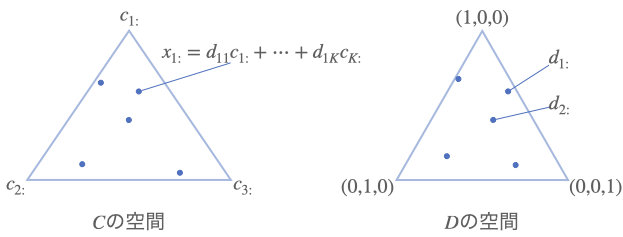
\includegraphics[width=\hsize]{d-space}
					\caption{$C$の空間と$D$の空間.}
					\label{fig:d-space}
			\end{center}
		\end{minipage}
    \begin{minipage}{0.3\hsize}
			\begin{center}
					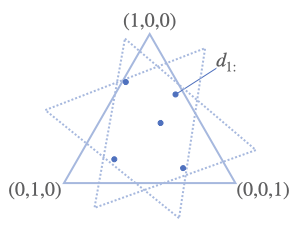
\includegraphics[width=\hsize]{d-rotate}
					\caption{$D$の空間の軸は回転・移動する.}
					\label{fig:d-rotate}
			\end{center}
		\end{minipage}
\end{figure}
\begin{figure}[htbp]
		\begin{center}
				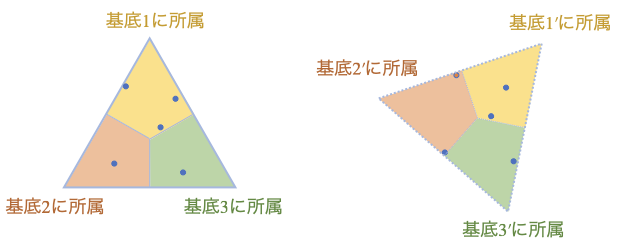
\includegraphics[width=0.8\hsize]{p-rotate}
				\caption{$D$の空間の軸の変化によってニューロンが所属する基底が変化する.}
				\label{fig:p-rotate}
		\end{center}
\end{figure}

\subsection{ブートストラップ法}
% アンサンブル学習の一つにバギング\cite{Breiman1996}がある.
ブートストラップ法\cite{Efron1979}とは,推定量の分布を近似する方法である.
データ$X$が分布$F$に従うとき,確率変数$R(X,F)$を推定する問題を考える.
ブートストラップサンプル$X^*$を作成して,$R^* = R(X^*, \hat{F})$を推定すると,$R^*$の分布は$R$の分布を近似する.

今回の問題ではブートストラップサンプル$X^*$から$A^*$を推定する.
類似度$A$を$A^*$の期待値$E[A^*|X]$として推定する:
\begin{align}
	A &= E[A^*|X] \\
	&=\frac{1}{B} \sum_{b=1}^B A^{*b},
\end{align}
ただし,$B$はブートストラップサンプル数,$A^{*b}$は$X^{*b}$から推定された推定量である.

NMFのブートストラップ方法にはいくつかの方法が考えられる.
簡単な3種類の方法について説明する.
列のサンプリングによるブートストラップは,データ行列$X$の各列がデータサンプルとしてみなせるので,列をサンプリングして$X^*$を作る方法である.
% \begin{align}
% 	X^* = \left[ X_{:sample(1,\dots,J)}, \cdots, X_{:sample(1,\dots, J)}\right],
% \end{align}
ブロックブートストラップでは,複数列を塊としてサンプリングする.
この方法は時系列データでのブートストラップで用いられており,時間方向に制約の入ったNMFなどでは有効である.
残差型ブートストラップは一回NMFのモデルを推定し,推定後の残差をサンプリングして推定した$DC$に足す方法である.
\begin{align}
	X^* = \hat{D} \hat{C} + H^*,
\end{align}
ただし,$\hat{D}$と$\hat{C}$は最優推定量で,$H^*$は$X - \hat{D}\hat{C}$をリサンプリングした行列である.
ニューロンごとにノイズの大きさが異なることが想定される場合は,行ごとにリサンプリングを行うのが適切だと考えられる.
NMFのモデル\eqref{eq:model_matrix}では$H$はi.i.d.なノイズという仮定を置いているので,残差型ブートストラップが一番モデルに沿ったブートストラップ方法と言える.

機械学習の分野でブートストラップ法が多く使われる場面はバギング\cite{Breiman1996}である.
バギングとは,ブートストラップ法によって学習器を増やしその出力の平均をとる学習方法である.
今回のブートストラップ法の使い方もバギングとして見ることができる.

\subsection{モデル平均}
モデル平均とは異なるモデルの推定量の平均をとって精度向上を測る方法である.
本論文で用いる推定量$A^*$は基底数によって行列サイズが変化しないので,異なる基底数の推定結果の平均をとることができる.
その場合の推定量は:
\begin{align}
	A = \frac{1}{K_{max} - K_{min} + 1} \sum_{k=K_{min}}^{K_{max}} A_k,
\end{align}
ただし,平均する最小の基底数を$K_{min}$,最大の基底数を$K_{max}$とする.

次節でも触れるが,NMFの真の基底数を求めるのは難しい問題である.
モデル平均によって,異なる基底数の推定結果を平均して精度をあまり落とさないようにする.
今回扱うデータから推定される$A$は基底数が違う時に大きくは変化しない.
真の基底数周りで平均した$A$の方が真の基底数でないモデルから推定された$A_k$よりも精度が落ちないと考えられる.

アンサンブル学習では,それぞれのモデルにある程度の推定精度があり\cite{Kittler1998},答えに多様性がある方が精度が上がる\cite{Kuncheva2006}と言われている.
本論文でのモデル平均の使い方は,真の基底数が分からない時に推定結果をなまして推定を間違うリスクを下げるという使い方をしている.

\subsection{NMFの基底数}
NMFの基底数の決め方にはいくつかのアプローチがある.
まずは,専門家や解析者の知識に基づいて決めることである.
この方法はデータに対して十分な知識がない時には使えない.

次にBIC~\cite{wasserman2000a}やAIC~\cite{Akaike1974}を用いる方法である.
これらは漸近理論に基づいた近似を行った情報量基準である.
NMFはデータが増えるほどパラメータ数$(I + J) * K$が増えるという特徴があり,これらを用いるのは本来不適切である.

次にRのNMFパッケージにも組み込まれているBrunetら~\cite{Brunet2004}の方法を紹介する.
彼らはNMFの推定結果からノード同士が同じ基底に所属するかしないかを表すconnectivity matrix $A \in \{0, 1\}^{I \times I}$を作成する.
本論文の推定量$A$と同じ意味の行列である.
初期値を20-100回変化させて$C$の平均$\bar{A} \in [0, 1]^{I \times I}$を計算する.
彼らは真の基底数ではこの推定量が$0$か$1$に寄るようになると仮定して,最も$\bar{A}$が安定する基底数を求める.
安定度は$1- \bar{A}$とそのcophenetic correlation coefficientのPearson correlationから計算する.

Ubaruら~\cite{Ubaru2017}はブートストラップを用いてNMFを行っており,$D$がそれほど変わらない基底数を採用している.
推定した$D_b$同士の相互相関行列についてdissimilarity~\cite{Wu}を測りその平均が最小となる基底数を用いる.

Hutchinsらはテストデータに対するRSS(residual sum of squares)が真の基底数以降になるとあまり下がらなくなると論じている\cite{Hutchins2008}.

Bayesian NMFではギブスサンプリングなどを用いてモデルエビデンスを計算している\cite{Cemgil2009}.

上記で述べた方法の他にも様々な方法が考案されているが,全てのデータに当てはめられるような枠組みは存在しない.


\section{$A$のクラスタリング}
$A$のクラスタリングにはスペクトラルクラスタリングを用いる.
スペクトラルクラスタリングは,グラフをクラスタリングする.
隣接行列からグラフラプラシアンを求め,その固有ベクトルをk-meansなどでクラスタリングする.
他のクラスタリング手法も使えるが,$A$をグラフとして見ることができるため,スペクトラルクラスタリングを用いる.
\subsection{スペクトラルクラスタリングのクラスタ数の決め方}
クラスタリングにおけるクラスタ数の決め方には様々な方法がある.
その中でもクラスタリング手法によらない方法は,安定性を見る方法\cite{Ben-Hur}やGap統計量\cite{Tibshirani}がある.
スペクトラルクラスタリングに特化した方法としては,固有値ギャップを見る方法\cite{VonLuxburg}がある.

固有値ギャップは固有値を小さい順にプロットした際に,一気に固有値が大きくなる箇所である.
そこをクラスタ数とする.
これは目で見て判断しなければならないが,今回は固有値の差分を取って大津の二値化にかけ,差分が大きいグループの最大の固有値の箇所を固有値ギャップとして計算した.

クラスタが明瞭な場合に固有値ギャップを見る方法が最も安定してクラスタ数を決定できたため,実験では固有値ギャップを見る方法を採用する.

\subsection{評価}
比較手法には\cite{Molter2018}で性能の良かったICA-CSを用いる.
また,相関行列とも比較を行う.

クラスタリングの評価方法には同論文で用いられていたBest Match scoreを用いる.
二つのクラスタリング結果$\mathcal{A} = \{A_1, \dots, A_{|\mathcal{A}|}\}$と$\mathcal{A^\prime} = \{A^\prime_1, \dots, A^\prime_{|\mathcal{A}^\prime|}\}$があった場合を考える.
$\mathcal{A}$と$\mathcal{A^\prime}$のBest Match distance~\cite{Goldberg2010}を
\begin{align}
	BestMatch_d = \sum_{A \in \mathcal{A}} min_{A^\prime \in \mathcal{A^\prime}} d(A, A^\prime) + \sum_{A^\prime \in \mathcal{A^\prime}} \min_{A \in \mathcal{A}} d(A^\prime, A),
\end{align}
とする.
ただし,
\begin{align}
	d(A,A^\prime) = 1 - \frac{|A \cap A^\prime|}{|A \cup A^\prime|},
\end{align}
である.
これはJaccard係数を1から引いた量である.
Best Match scoreは
\begin{align}
	Best Match score = 1 - \frac{1}{|\mathcal{A}| + |\mathcal{A^\prime}|} BestMatch_d(\mathcal{A}, \mathcal{A^\prime}),
\end{align}
である.
